\documentclass[conference]{IEEEtran}
\IEEEoverridecommandlockouts

\usepackage{cite}
\usepackage{amsmath,amssymb}
\usepackage{graphicx}
\usepackage{booktabs}
\usepackage{url}
\usepackage[hidelinks]{hyperref}

% This TeX installation (BasicTeX) ships Times but not the URW Courier or
% Helvetica metrics, and tlmgr cannot fetch them across a release boundary.
% Times remains the body face, which is what the IEEE template requires; only
% verbatim text falls back to Computer Modern Typewriter.
\renewcommand{\ttdefault}{cmtt}
\renewcommand{\sfdefault}{cmss}
\urlstyle{same}

\begin{document}

\title{Requested Is Not Realised: Measuring Rate Adherence\\
and Output Expansion in Neural Prompt Compression}

\author{\IEEEauthorblockN{Author Name}
\IEEEauthorblockA{\textit{Department Name} \\
\textit{Institution Name}\\
City, Country \\
author@institution.edu}
}

\maketitle

\begin{abstract}
Prompt compression lowers the cost of large language model inference, but
deployed compressors take the compression rate as a hyperparameter supplied by
the user and applied uniformly to inputs that tolerate compression very
differently. We report a controlled measurement of what a requested rate
actually delivers. Using LLMLingua-2 as the compressor and a local
instruction-tuned 3B target model, we run a 630-cell grid over 30 instances
from three task families and seven compression budgets, plus a separate
1{,}044-point sweep over 174 instances that requires no target-model calls.
Three results follow. First, the realised compression rate is consistently
below the requested one when measured in the target model's tokenizer, with a
signed error between $-0.025$ and $-0.053$ whose bootstrap confidence
intervals all exclude zero; the error varies non-monotonically with the
requested budget and differs by a factor of about three across task families,
so it is not correctable by a single scalar offset. Second, compression
increases output length on two of three families, but the increase does not
change the cost-optimal budget: across all 25 evaluable instances and output
price ratios from 1 to 5, the cheapest safe budget was always the smallest
safe budget, because input reduction exceeds output growth by roughly two
orders of magnitude in short-answer tasks. Third, per-instance heterogeneity
in compression tolerance is visible in the measured curves but is not
statistically resolvable at three samples per cell; an extrapolation from the
measured noise floor indicates that roughly twenty samples per cell are
required. The last result is a constraint on experimental design for this line
of work rather than a finding about compression itself. All measurements come
from a single target model and a single compressor checkpoint.
\end{abstract}

\begin{IEEEkeywords}
prompt compression, large language models, inference cost, measurement,
experimental design
\end{IEEEkeywords}

\section{Introduction}

Prompt compression reduces the number of input tokens sent to a large language
model by deleting or rewriting parts of the prompt. Token-level methods such
as LLMLingua \cite{jiang2023llmlingua} and its successors
\cite{jiang2024longllmlingua,pan2024llmlingua2} now achieve large reductions
with modest quality loss, and the compression rate is the primary control the
user has over the resulting trade-off.

That control is weaker than it appears, in two ways that this paper measures.

The first concerns what the rate actually means. A compressor is asked for a
rate $b$ and returns text whose realised rate $r$ is measured after the fact.
If $r \neq b$ systematically, then a reported saving computed from $b$
describes a request rather than a result. Prior work has observed that
adherence is imperfect \cite{kummer2026wild}; we characterise its structure
across budgets and task families, measured in the tokenizer of the model that
is actually billed.

The second concerns what the objective should be. Providers bill input and
output tokens separately, and output tokens usually cost more. Compression
changes output length as well as input length, and under aggressive truncation
that change can be large \cite{johnson2026method}. If output growth is large
enough, then a more aggressive budget can be both quality-safe and more
expensive, which would make the common rule of taking the smallest safe budget
incorrect. Whether that happens is an empirical question about the
output-to-input token ratio in a given workload, and we test it directly.

Our contributions are measurements rather than a method:

\begin{enumerate}
\item A characterisation of LLMLingua-2 rate adherence in the target
tokenizer, over 1{,}044 measurements and 174 instances, showing a consistent
negative signed error with a non-monotonic dependence on the requested budget
and a factor-of-three spread across task families.
\item A test of whether compression-induced output expansion changes the
cost-optimal budget. Expansion is present, but the optimum does not move in
any of the 25 evaluable instances at output price ratios from 1 to 5. We
report this bounded negative alongside the positive expansion measurement.
\item A power analysis of per-instance frontier estimation, showing that the
sampling noise floor, and not the number of instances, is the binding
constraint, and quantifying the samples per cell required to clear it.
\end{enumerate}

We do not propose a compression method, a rate predictor, or a selection
policy, and we make no claim about model families other than the one measured.

\section{Related Work}

\textbf{Compression methods.} LLMLingua \cite{jiang2023llmlingua} allocates a
user-specified budget across prompt segments using a small language model's
perplexity. LongLLMLingua \cite{jiang2024longllmlingua} adds question-aware
coarse-to-fine selection for long contexts. LLMLingua-2
\cite{pan2024llmlingua2} reframes compression as binary token classification
with a bidirectional encoder distilled from GPT-4 annotations, and is both
faster and more robust out of domain, which is why we use it here. In all
three the rate is supplied by the user.

\textbf{Adaptive rate selection.} AdaComp \cite{zhang2024adacomp} predicts how
many retrieved documents to keep, at document granularity in a
retrieval-augmented setting. Guo et al. \cite{guo2025adaptive} adapt
compression to input complexity at embedding granularity. Nagle et al.
\cite{nagle2024limits} characterise the fundamental distortion-rate limit of
prompt compression with oracle access, which bounds what any selector could
achieve rather than providing one. These works motivate per-instance rate
selection; none of them reports the adherence gap between requested and
realised rates.

\textbf{Cost and latency in deployment.} Kummer et al. \cite{kummer2026wild}
present a large-scale study of compression overhead against decoding latency
across several open models and three GPU classes, and report end-to-end
speedups only inside a matched operating window of prompt length, rate and
hardware. Their study includes rate adherence among the quantities measured,
so we do not claim priority for observing it; our contribution is the shape of
the error as a function of the requested budget and its variation across task
families, measured in the target tokenizer. Johnson
\cite{johnson2026production,johnson2026method} reports that aggressive
compression can raise total cost through output expansion, with a strong
benchmark effect (a reported 56$\times$ expansion on MBPP against 5$\times$ on
HumanEval). That work uses truncation as the compression operator and studies
code generation. We measure expansion with a neural compressor and task-native
metrics, and we find that in short-answer question answering the effect does
not reach the threshold needed to move the cost optimum.

\textbf{Risk control.} Distribution-free risk control
\cite{angelopoulos2022crc,angelopoulos2021ltt} and its application to
prompting decisions \cite{zollo2023prc} offer a route to calibrated rate
selection. We cite this line as context for future work; no guarantee is
constructed or claimed in this paper.

\section{Method}

\subsection{Definitions}

An instance is a pair $(x,q)$ of context and query. A compressor $\psi$ takes
a requested budget $b \in (0,1]$ and returns compressed context
$\psi(x,q,b)$. The realised rate is
\begin{equation}
r(x,q,b) = \frac{|T(\psi(x,q,b))|}{|T(x)|},
\end{equation}
where $T$ is the \emph{target model's} tokenizer. Measuring $r$ in the
compressor's own tokenizer would report a quantity that does not determine the
bill; the two disagree, and the target-side count is the one that is charged.
The adherence error is the signed quantity $r - b$.

Quality $\rho(x,b) \in [0,1]$ is the task metric, estimated by averaging over
$k$ stochastic generations. Because $\rho$ is estimated, every per-instance
quantity derived from it carries sampling noise, which Section
\ref{sec:power} treats explicitly.

\subsection{Cost model}

Total cost in token units is
\begin{equation}
C(x,b) = T_{\mathrm{in}}(x,b) + \gamma \, T_{\mathrm{out}}(x,b),
\qquad \gamma = c_{\mathrm{out}}/c_{\mathrm{in}}.
\label{eq:cost}
\end{equation}
Local inference has no provider bill, so USD in our ledger is zero by
construction. We therefore report cost in token units under an explicit
$\gamma$ and sweep $\gamma \in \{1,\dots,5\}$, which states conclusions as a
function of the price ratio rather than of one vendor's price list.

Given a tolerance $\varepsilon$, the safe set at instance $x$ is
$\mathcal{B}(x) = \{b : \rho(x,b') \geq \rho(x,1) - \varepsilon \ \ \forall b'
\geq b\}$, defined over the suffix so that a single noisy dip does not
certify an aggressive budget as safe. The two candidate rules are the smallest
safe budget $\min \mathcal{B}(x)$ and the cheapest safe budget $\arg\min_{b
\in \mathcal{B}(x)} C(x,b)$. They coincide whenever $C$ is increasing in $b$;
they differ only if output growth outweighs input reduction. We measure how
often they differ.

\subsection{Statistics for heterogeneity}
\label{sec:power}

The quantity of interest for per-instance rate selection is whether instances
differ in compression tolerance by more than estimation noise. The natural
label, the smallest safe budget $b^{*}$, is a threshold crossing of a noisy
curve and inherits the noise of every budget it crosses. We therefore also
report a smoother statistic, the compression sensitivity
\begin{equation}
S(x) = \rho(x,1.0) - \rho(x,0.2),
\end{equation}
which uses only the two endpoints and is better conditioned at small $k$.

For both statistics we estimate a sampling noise floor by split-half
resampling: the $k$ generations of each instance are split in two, the
statistic is computed on each half, and the mean squared half-difference
divided by two estimates the variance attributable to sampling. Heterogeneity
is declared only if the bootstrap lower bound on the between-instance variance
exceeds twice this floor.

Instances with $\rho(x,1) = 0$ are excluded from these tests. A prompt the
model already fails without compression has no compression tolerance to
measure: every budget trivially satisfies the safety condition, so its $b^{*}$
reflects model failure rather than compression behaviour.

\section{Experimental Setup}

\begin{table}[t]
\caption{Experimental configuration. All values are recorded in the run
manifest committed with the ledger.}
\label{tab:setup}
\centering
\small
\begin{tabular}{ll}
\toprule
Compressor & LLMLingua-2, CPU backend \\
Checkpoint & {\footnotesize\texttt{bert-base-multilingual-cased-}} \\
 & {\footnotesize\texttt{meetingbank}} \\
Target model & Llama-3.2-3B-Instruct, Q4\_K\_M, Ollama \\
Context window & 8192 tokens, enforced \\
Budgets $b$ & 1.0, 0.8, 0.65, 0.5, 0.4, 0.3, 0.2 \\
Samples $k$ & 3 per cell, temperature 0.7, seeds 0--2 \\
Families & MultiFieldQA (F1), 2WikiMQA (F1), \\
 & GSM8K (exact match) \\
Instances & 10 per family, 30 total \\
Grid & 630 cells, 0 failures \\
Adherence sweep & 1{,}044 points, 174 instances, 6 budgets \\
Context length & 500--3500 tokens (selection window) \\
Tolerance & $\varepsilon = 0.05$ \\
\bottomrule
\end{tabular}
\end{table}

Table \ref{tab:setup} summarises the configuration. The three families are
drawn from LongBench (MultiFieldQA-en, 2WikiMQA) and GSM8K. MultiFieldQA and
2WikiMQA are scored with token-level F1; GSM8K uses exact match on the
extracted numeric answer, and its context is the few-shot exemplar block,
which is the setting LLMLingua-2 itself targets.

Instances were restricted to contexts between 500 and 3500 tokens. Families
whose natural length exceeds the target's usable window, specifically HotpotQA
(median 14{,}114 tokens) and QMSum (13{,}505), were excluded rather than
truncated to fit. Truncating them would remove the supporting passage and
force $\rho(x,1) = 0$, producing degenerate labels for a reason unrelated to
compression.

Two controls matter for interpretation. The harness raises an error if the
server reports that the prompt reached the context ceiling, because silent
truncation at $b = 1.0$ would contaminate the reference quality against which
every frontier is measured. Token counts are taken from the server's reported
usage rather than from local re-tokenisation.

The realised rate is measured with a GPT-2 byte-pair tokenizer as a proxy,
since the Llama-3.2 tokenizer is gated. This shifts the absolute level of the
adherence error but not its ordering across budgets; the substitution is
recorded in the run manifest.

Confidence intervals are bootstrap percentile intervals over instances with
10{,}000 resamples. The grid consumed 1.28 hours of measured wall time on an
Apple M3 with 16\,GB of unified memory, of which compression accounted for
23.4\%.

\section{Results}

\subsection{Which families support quality conclusions}

\begin{table}[t]
\caption{Mean quality against requested budget, by family. MultiFieldQA and
2WikiMQA are token-F1; GSM8K is exact match. Each cell averages 30
generations (10 instances $\times$ 3 samples).}
\label{tab:quality}
\centering
\small
\begin{tabular}{cccc}
\toprule
$b$ & MultiFieldQA & 2WikiMQA & GSM8K \\
\midrule
1.00 & 0.544 & 0.105 & 0.467 \\
0.80 & 0.552 & 0.101 & 0.633 \\
0.65 & 0.534 & 0.101 & 0.633 \\
0.50 & 0.431 & 0.096 & 0.567 \\
0.40 & 0.432 & 0.072 & 0.667 \\
0.30 & 0.377 & 0.071 & 0.533 \\
0.20 & 0.333 & 0.064 & 0.667 \\
\bottomrule
\end{tabular}
\end{table}

\begin{table}[t]
\caption{Validity preconditions per family. An instance is solvable if
$\rho(x,1) > 0$; unsolvable instances have no compression tolerance to
measure. Only MultiFieldQA satisfies both preconditions.}
\label{tab:validity}
\centering
\small
\begin{tabular}{lccl}
\toprule
Family & solvable & $\rho(x,1)$ & status \\
\midrule
MultiFieldQA & 10/10 & 0.544 & usable \\
2WikiMQA & 9/10 & 0.105 & near-floor accuracy \\
GSM8K & 6/10 & 0.467 & 4 degenerate instances \\
\bottomrule
\end{tabular}
\end{table}

Table \ref{tab:quality} gives the measured quality curves and Table
\ref{tab:validity} the preconditions that determine which of them can be
interpreted. Two of the three families are compromised as quality
measurements, for different reasons, and we state this before reporting
quality results rather than after.

On 2WikiMQA the target model scores 0.105 uncompressed. At that level the
model is close to the floor of the metric and the curve is nearly flat across
the whole budget range (0.105 down to 0.064), so there is little quality to
lose and no informative frontier. On GSM8K, 4 of 10 instances are not solved
at $b=1.0$ in any of the three samples; for those instances every budget
trivially satisfies the safety condition, and their $b^{*}$ records model
failure rather than compression tolerance. The GSM8K column of Table
\ref{tab:quality} is also visibly non-monotone: its highest values (0.667)
occur at $b=0.4$ and $b=0.2$ and its lowest (0.467) at $b=1.0$. At $k=3$ on a
binary metric this is consistent with sampling noise rather than with
compression improving accuracy.

MultiFieldQA satisfies both preconditions, and its curve declines
monotonically apart from a small rise at $b=0.8$. Quality conclusions in the
remainder of this section therefore rest on MultiFieldQA. The adherence
result in Section \ref{sec:adh} does not depend on generation at all and is
unaffected by these preconditions.

\subsection{Rate adherence}
\label{sec:adh}

\begin{table}[t]
\caption{Requested against realised compression rate, pooled over three
families ($n=174$ instances per budget). All confidence intervals exclude
zero.}
\label{tab:adherence}
\centering
\small
\begin{tabular}{ccccc}
\toprule
$b$ & realised $r$ & s.d. & $r-b$ & 95\% CI \\
\midrule
0.20 & 0.1751 & 0.0104 & $-0.0249$ & $[-0.0265, -0.0233]$ \\
0.30 & 0.2656 & 0.0143 & $-0.0344$ & $[-0.0365, -0.0323]$ \\
0.40 & 0.3581 & 0.0190 & $-0.0419$ & $[-0.0448, -0.0391]$ \\
0.50 & 0.4492 & 0.0196 & $-0.0508$ & $[-0.0538, -0.0479]$ \\
0.65 & 0.5973 & 0.0271 & $-0.0527$ & $[-0.0568, -0.0487]$ \\
0.80 & 0.7596 & 0.0327 & $-0.0404$ & $[-0.0453, -0.0355]$ \\
\bottomrule
\end{tabular}
\end{table}

\begin{figure}[t]
\centering
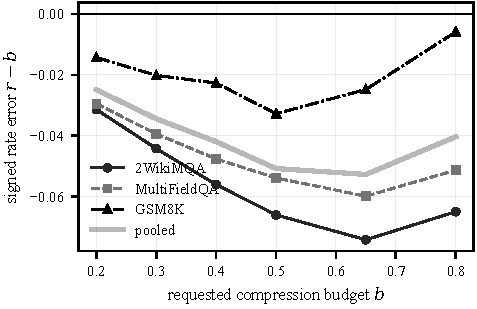
\includegraphics[width=\columnwidth]{figures/fig_adherence.pdf}
\caption{Signed rate error $r-b$ against requested budget, by family and
pooled. The error is negative at every budget, is largest in magnitude near
$b=0.65$, and differs by roughly a factor of three between 2WikiMQA and
GSM8K.}
\label{fig:adherence}
\end{figure}

LLMLingua-2 returns less text than requested at every budget tested. Table
\ref{tab:adherence} gives the pooled measurement and Fig.
\ref{fig:adherence} shows its structure. Two features are relevant to anyone
using the requested rate as a control variable.

The error is not constant. It grows from $-0.025$ at $b=0.2$ to $-0.053$ at
$b=0.65$ and then shrinks to $-0.040$ at $b=0.8$, an inverted-U shape in the
requested budget. A single additive or multiplicative correction therefore
cannot remove it.

The error is family-dependent. At $b=0.65$ the mean signed error is $-0.074$
on 2WikiMQA, $-0.060$ on MultiFieldQA and $-0.025$ on GSM8K. The dependence on
input text, and not only on the requested budget, is what would make a learned
per-instance correction the appropriate object rather than a lookup table.

In absolute terms these errors are modest: at most about 5 percentage points
of the original prompt. They matter because they are systematic and
directional, not because any single instance is badly served. A saving
reported as $1-b$ overstates the compression achieved in every condition we
measured.

\subsection{Output expansion and the cost optimum}

\begin{figure}[t]
\centering
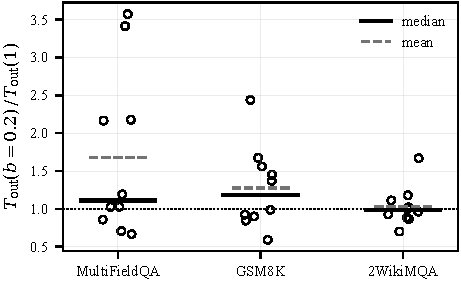
\includegraphics[width=\columnwidth]{figures/fig_expansion.pdf}
\caption{Per-instance output expansion at $b=0.2$ relative to $b=1.0$. Each
circle is one instance. The distribution is heavy-tailed on MultiFieldQA: the
mean (dashed) is pulled well above the median (solid) by four instances, while
three others contract.}
\label{fig:expansion}
\end{figure}

Compression lengthens model output on two of the three families. At $b=0.2$
the mean ratio $T_{\mathrm{out}}(0.2)/T_{\mathrm{out}}(1)$ is 1.681
(95\% CI $[1.268, 2.135]$) on MultiFieldQA and 1.275 ($[1.086, 1.481]$) on
GSM8K, both excluding 1.0. On 2WikiMQA the ratio is 1.033
($[0.889, 1.177]$), which does not exclude 1.0.

The mean is a poor summary here, and Fig. \ref{fig:expansion} shows why. On
MultiFieldQA the ten per-instance ratios are heavy-tailed: the median is 1.110,
four instances exceed 1.2 (reaching 2.17, 2.18, 3.41 and 3.57), and three
instances contract to 0.67, 0.71 and 0.86. The effect is real in the mean but
concentrated in a minority of instances at $n=10$, and we treat the magnitude
as exploratory rather than well estimated.

Whether expansion matters for cost depends on the magnitudes involved. On
MultiFieldQA, moving from $b=1.0$ to $b=0.2$ reduces input from 2405 to 498
tokens, a saving of 1907, while output rises from 29.5 to 39.9 tokens, an
increase of 10.4. Even at $\gamma = 5$ the comparison is 1907 against 52.

Applying the test of Section \ref{sec:power} directly: across all 25 instances
with a non-empty safe set, at every price ratio $\gamma \in \{1,2,3,4,5\}$,
the cheapest safe budget equalled the smallest safe budget. The divergence
rate is 0 of 25 in every condition.

This is a bounded negative result, and it does not contradict the reported
compression paradox \cite{johnson2026method}. That work measured code
generation under truncation, where outputs are long relative to inputs and
expansion factors reach 56$\times$. The mechanism requires a high
output-to-input token ratio. In short-answer question answering the ratio is
roughly 1:80, and an expansion of even 1.68$\times$ cannot overcome it. The
practical statement is conditional: optimising the smallest safe budget is
adequate for short-output workloads, and the cheapest-safe rule is worth its
extra complexity only when outputs are long relative to inputs.

\subsection{Per-instance heterogeneity is not resolvable at $k=3$}

\begin{figure}[t]
\centering
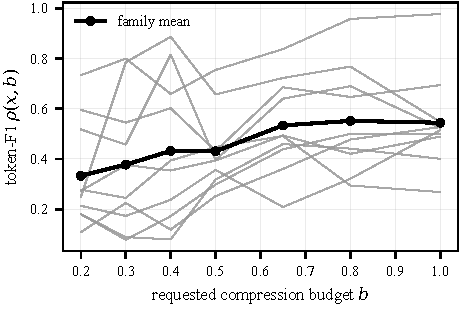
\includegraphics[width=\columnwidth]{figures/fig_frontiers.pdf}
\caption{Per-instance quality against requested budget on MultiFieldQA, the
one family with no validity problems. Grey lines are individual instances,
black is the family mean. The spread between instances is visible; Section
\ref{sec:power} shows it is not separable from sampling noise at $k=3$.}
\label{fig:frontiers}
\end{figure}

\begin{table}[t]
\caption{Heterogeneity test on compression sensitivity $S(x)$, restricted to
instances solvable without compression. No family clears the criterion at
$k=3$. Required $k$ extrapolates the floor as $\propto 1/k$ and is an estimate,
not a measurement.}
\label{tab:power}
\centering
\small
\begin{tabular}{lccccc}
\toprule
Family & $n$ & mean $S$ & $\mathrm{Var}[S]$ & floor & required $k$ \\
\midrule
MultiFieldQA & 10 & $+0.211$ & 0.0194 & 0.0655 & 20 \\
2WikiMQA & 9 & $+0.049$ & 0.0022 & 0.0052 & 14 \\
GSM8K & 6 & $-0.056$ & 0.1519 & 0.1690 & 7 \\
\bottomrule
\end{tabular}
\end{table}

Fig. \ref{fig:frontiers} shows the per-instance frontiers on MultiFieldQA, the
only family that passes all validity preconditions (10 of 10 instances
solvable uncompressed, $\rho(x,1) = 0.544$). The instances visibly differ: one
declines from 0.98 to 0.73 across the budget range while another falls from
0.53 to 0.11.

That visible spread is nevertheless not statistically separable from sampling
noise. Pooled over families, $\mathrm{Var}[b^{*}] = 0.108$ with bootstrap CI
$[0.074, 0.133]$ against a noise floor of 0.055, so the interval straddles the
$2\times$ floor criterion. Table \ref{tab:power} repeats the test on the
better-conditioned sensitivity statistic, and no family clears it.

The binding constraint is $k$, not $n$. The noise floor of a per-instance mean
scales approximately as $1/k$, so the samples per cell needed for the observed
between-instance variance to exceed twice the floor can be estimated. For
MultiFieldQA that estimate is $k \geq 20$. This is an extrapolation from a
floor measured at $k=3$ and should be treated as a design estimate rather than
a measured quantity.

The metric choice interacts with this. The exact-match floor on GSM8K is
0.1690 against 0.0655 for token-F1 on MultiFieldQA. Graded metrics carry
roughly 2.5 times less per-instance sampling noise than binary ones at equal
$k$, so a graded metric buys statistical power at no additional sampling cost.

\subsection{Curve shape}

Naive and suffix-safe definitions of $b^{*}$ disagree on 20.0\% of the 30
instances, with a mean gap of 0.483 in budget units. Aggregate quality peaks
at $b = 0.8$ (0.428) rather than at $b = 1.0$ (0.372). We do not read the
latter as compression improving accuracy; with $k=3$ it is within the range
that sampling noise produces, and it is one of the two conditions that make
the pooled Gate-1 verdict uninterpretable. It does establish that the measured
curves are not monotone, which is why a suffix-based safety definition is
preferable to taking the smallest budget that happens to satisfy the tolerance.

\section{Discussion}

The three results differ in how much weight they can carry.

Rate adherence is well powered and consistent, resting on 1{,}044 measurements
with no target-model calls, and every interval excludes zero. Its practical
consequence is narrow but concrete: the requested rate is a request, and
reported savings computed from it are biased in a known direction.

The cost result is a conditional negative. Expansion exists and is significant
in the mean, but it does not move the optimum for this workload, and the
reason is a token-ratio argument that transfers to other short-output tasks.
Reporting the 1.68$\times$ expansion without the 0-of-25 divergence would
reproduce, with the sign reversed, the reporting problem this work set out to
examine.

The power result is the one that most changes what should be done next. The
absence of a heterogeneity finding here is a statement about sample size, not
about compression. Any study that estimates per-instance compression
frontiers, then selects a rate from them, needs enough samples per cell for
the per-instance label to be meaningful, and $k=5$ is a common choice that our
measurement suggests is too small for graded QA metrics by roughly a factor of
four.

\subsection{The experiment that would settle the open question}

The power analysis specifies its own follow-up. Holding the instance count at
ten and raising the sample count to $k=20$ on MultiFieldQA gives 1{,}400
cells, which at the 7\,s per cell measured here is about three hours on the
same hardware. That design keeps every other factor fixed and moves only the
quantity our analysis identifies as binding.

Either outcome is informative. If the between-instance variance then exceeds
twice the recomputed floor, per-instance heterogeneity is established for this
family and per-instance rate selection has a measured basis. If it does not,
the result is a well-powered negative: compression tolerance on this task and
model would be close enough to uniform that a per-family fixed budget is the
appropriate policy, and the predictor machinery that motivated this line of
work would not be worth building. The present study cannot distinguish these
cases, which is the honest summary of its heterogeneity result.

\section{Limitations}

The scope of every claim is one target model, one compressor checkpoint, and
one context-length window.

\textit{Single model.} All quality and output-length measurements use
Llama-3.2-3B-Instruct at 4-bit quantisation. Output-length response to
compression is known to be model-dependent \cite{zhang2025empirical}, so the
expansion direction should not be generalised.

\textit{Single compressor.} Only LLMLingua-2 with the multilingual BERT-base
checkpoint was run. Adherence behaviour is a property of the compressor and
may not transfer. The checkpoint is trained on MeetingBank; none of our three
families is MeetingBank, so the results are out of domain for the compressor,
which we regard as the appropriate default.

\textit{Sample size.} Thirty instances at $k=3$ supports the adherence result,
which does not depend on generation, but is underpowered for heterogeneity and
gives wide intervals on expansion. The expansion magnitude in particular rests
on ten instances with a heavy-tailed distribution.

\textit{Task coverage.} As Table \ref{tab:validity} shows, quality
conclusions rest on MultiFieldQA alone, so they are supported by ten
instances. Excluding HotpotQA and QMSum for length means long-context
behaviour, which is where compression is most often deployed, is untested.

\textit{Tokenizer proxy.} Realised rate uses a GPT-2 tokenizer rather than the
target's, which shifts the absolute level of the adherence error.

\textit{Cost model.} Local inference is zero-priced, so all cost statements
are in token units under an assumed price ratio, and exclude compressor
compute. Kummer et al. \cite{kummer2026wild} show that compressor overhead can
cancel end-to-end gains outside a matched operating window; our token-unit
accounting does not capture that.

\textit{Runtime dependence.} Two measurements affect reproduction rather than
interpretation. Running the compressor on the Apple GPU backend was about
17 times faster than CPU (0.54\,s against 9.42\,s mean per compression), but
GPU residency of the compressor alongside the target model caused memory
pressure that terminated an earlier run, so the reported grid used the CPU
backend. Separately, issuing generation requests concurrently reduced
throughput on this single-GPU machine (12.0\,s per cell at one worker against
16.8\,s at four) because concurrent prefills contend for the same device;
prefill-bound workloads of this kind do not benefit from request-level
parallelism.

\textit{No method.} No predictor, selection policy or risk guarantee was
built or evaluated. Statements about what a learned adherence correction would
buy are hypotheses.

\section{Conclusion}

We measured what a requested compression rate delivers. For LLMLingua-2 on a
3B target model, the realised rate is consistently below the requested rate,
by an amount that varies non-monotonically with the budget and by a factor of
about three across task families; savings quoted from the requested rate are
therefore optimistic in a systematic way. Compression lengthens output on two
of three families, significantly so in the mean, but the increase never
changed the cost-optimal budget in our data, because input reduction dominates
output growth by about two orders of magnitude in short-answer tasks. The
smallest-safe-budget rule is adequate for such workloads; the distinction
matters only where outputs are long relative to inputs.

We could not establish per-instance heterogeneity in compression tolerance.
The curves show visible spread, but at three samples per cell it is not
separable from sampling noise, and our estimate is that roughly twenty samples
per cell would be needed for graded QA metrics. That is the main obstacle to
per-instance rate selection that this study identifies, and addressing it is a
precondition for the predictor and calibration work that motivated the
measurement.

\section*{Reproducibility}

The ledger, the analysis scripts and the figure-generation code are released
with the paper. Every number reported here is regenerated from
\texttt{runs/real\_v1/ledger.jsonl} and
\texttt{runs/adherence\_v1/adherence.csv} by the included scripts. The test
suite accompanying the harness passes 136 tests with 5 skipped.

\bibliographystyle{IEEEtran}
\bibliography{refs}

\end{document}
